\chapter{本学科领域的发展现状与趋势}
随着量子计算硬件规模的快速增长,量子电路的验证成为一个重要问题。开始的研究主要集中在BDD在量子计算下的推广算法,如量子信息决策图(Quantum Information Decision Diagram,或QuIDD)\citep{Viamontes_2003},量子多值决策图(Quantum multiple-valued Decision Diagram,或QMDD)\citep{Seiter_2013}等,从而对组合式量子电路进行等效性检查。显然,随着越来越复杂的物理可实现化的硬件出现,将会出现更加复杂的,更加针对于的,新的验证问题。比如量子存储\citep{Kerckhoff_2010},量子反馈网络\citep{Gough_2008},RUS量子电路\citep{Bocharov_2015}。量子模型检测可以为量子电路的验证提供了更多思路。

量子系统模型检测的早期工作旨在验证量子通信协议\citep{Gay,BALTAZAR_2008,davidson2012model}。后来还有针对分析和验证量子程序的应用\citep{ying2016foundations},比如量子自动机\citep{ying2014model}、量子马尔可夫链\citep{Ying_2013}和超算符值马尔可夫链\citep{feng2013model}的模型检测技术。然而,在这些量子模型检测技术与它们在验证量子电路方面实际应用之间存在巨大差距仍需填补。TDD作为新的数据结构,极大加快了计算过程,有可能深化二者的联系,加快实际应用的出现。
\section{发展现状}
TDD是一种相对较新的数据结构,用于表示和操作张量网络。张量网络提供了量子线路更紧凑的表现形式。在张量网络领域,目前除了TDD外目前还有直接使用张量网络,以及ZX-calculus\citep{van2020zx}。
图\ref{fig:zx-basic}展示了ZX-calculus中量子计算基本门的形式。图\ref{fig:zx-rule}展示了ZX-calculus的基本化简规则。将一个量子线路中的比特门表示为Z-calculus后化简,从而进行验证。

\begin{figure}[!htbp]
    \centering
    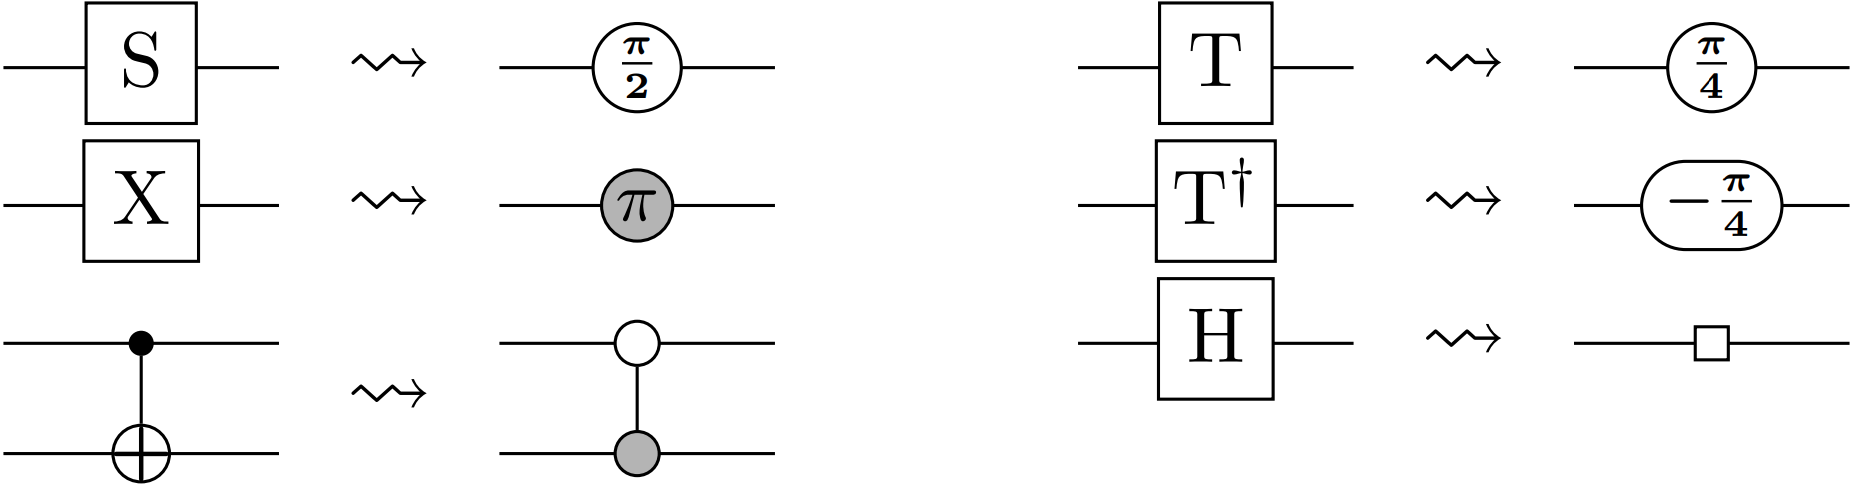
\includegraphics[height=4cm]{Img/zx-basic.pdf}
    \caption{量子计算基本门在ZX-calculus的表示}
    \label{fig:zx-basic}
\end{figure}
\begin{figure}[!htbp]
    \centering
    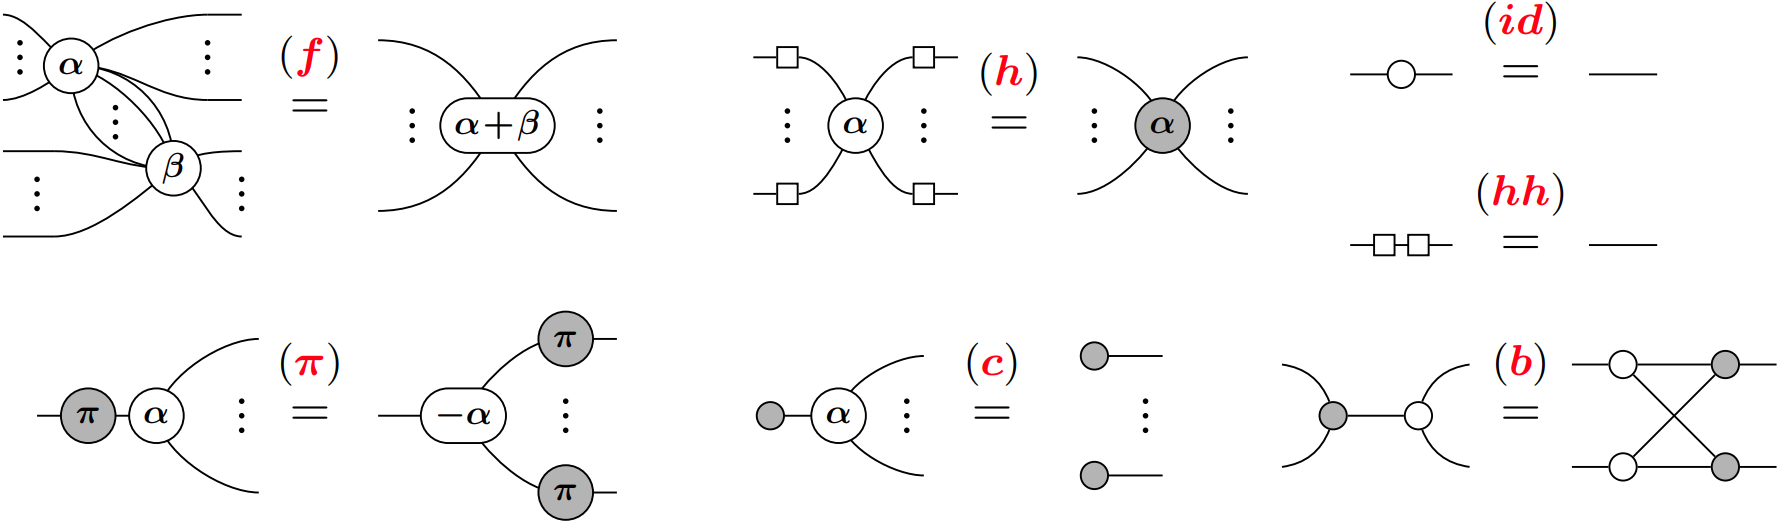
\includegraphics[height=4cm]{Img/zx-rule.pdf}
    \caption{ZX-calculus的基本化简规则}
    \label{fig:zx-rule}
\end{figure}
 
目前ZX-calculus发展还比较早期。图\ref{fig:tdd-compare}展示了目前各种比较成熟的表示方法下模拟量子电路的时间对比。其中TN是指google的tensor network。可以看到TDD相比其他有一定优势。因此本次研究选择TDD作为主要技术。

\begin{figure}[!htbp]
    \centering
    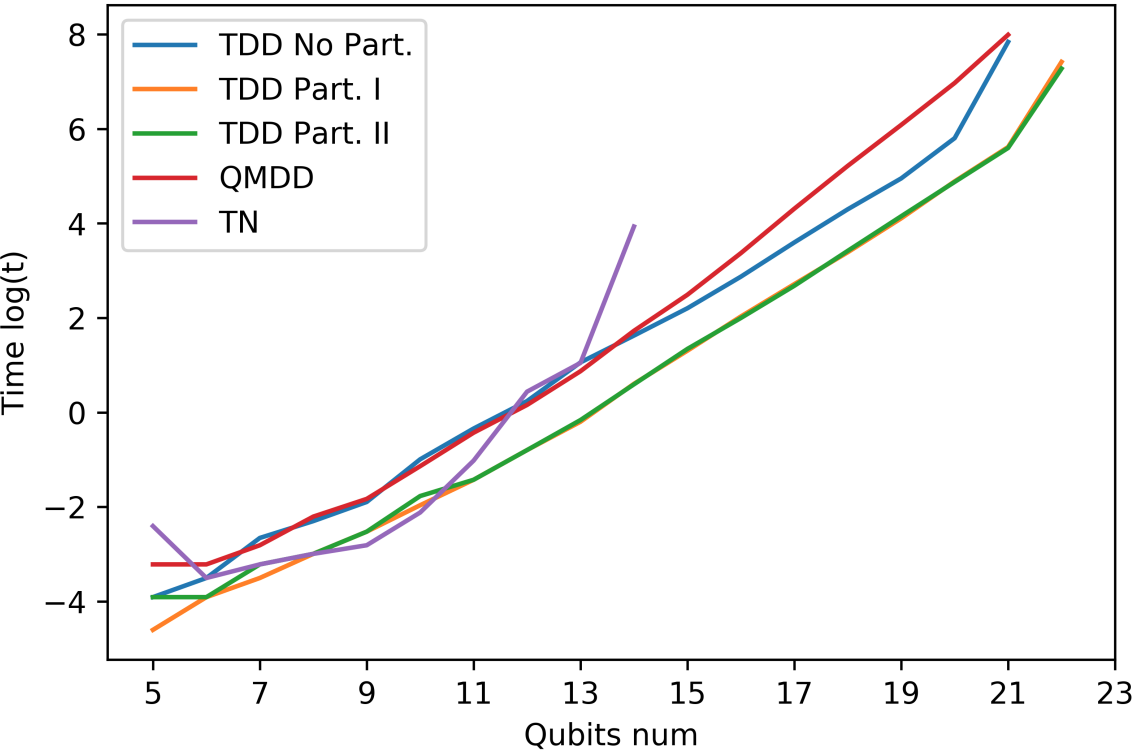
\includegraphics[height=5cm]{Img/tdd-compare.pdf}
    \caption{TDD与其他实验方法的比较\citep{Hong_2022}}
    \label{fig:tdd-compare}
\end{figure}

目前,TDD研究集中在开发更有效的算法来使用TDD操作和收缩张量网络。这包括开发新技术来分割张量网络,优化TDD结构,从而进一步提高基于TDD的可达性分析和模型检测算法的效率。这也是实现基于TDD的量子模型检测的主要方法。
\section{研究趋势}
未来量子模型检测的最重要目标是寻找一类更简单易于检测的属性。过去的研究追求的是普遍性,即只针对检查量子系统的一般可达性和时间逻辑属性。然而,为了实现这一目标,模型检测的效率非常低,且仅适用于非常小规模和深度较小的量子电路。因此,需要确定一类更简单易于检测的属性,以便当前的量子模型检测工具可以高效地进行检测\citep{ying2021model}。
这需要更多在时序逻辑上的研究工作。但同时更实用的模型检测工具也能在研究相关属性起到一定帮助。
% //TODO: QDA